\apphead{Corpus and evaluation apparatus}{app:eval}

What the corpus is made of beyond the counts \S\ref{sec:evaluation} quotes, how the
feature-coverage order is computed, and the two subsections that report what the
evaluation does \emph{not} establish. The body carries the answers; this carries the
characterisation a reader would need to disagree with them.

\begin{remark}[Two definitions in one comparison]\label{rem:template-shares}
The two template-variable shares beside the parse rates are now the same quantity, and
were not. The Datadog figure used to read $87\%$, which is the share of queries with a
variable \emph{inside a scope} and not the share with a variable at all, while the PromQL
figure beside it was the latter --- two definitions in one comparison, and the narrower
one on the side the sentence was about. A comparison between two languages is the place a
definitional slip is hardest to see, because the number it produces is of the right order
and points the way the argument already pointed.
\end{remark}

\begin{remark}[Three counts that moved on a seventh reading of the extractor]\label{rem:extraction-fixes}
Three of those counts moved in the seventh reading of the extractor, and in the direction
that costs an excuse rather than buying one: a request may carry its query as a singular
object rather than in a list, which distribution widgets do and which hid four Datadog
queries; a Grafana library panel keeps its model in the dashboard's \texttt{\_\_elements}
map rather than in \texttt{panels}, which hid four more; and \emph{two} of what had been
eleven LogQL panels were PromQL alerting rules whose only offence was a backtick raw
string in a matcher, which PromQL permits and a LogQL line-filter pattern matched.
\end{remark}

\paragraph{What is held aside.}
A Datadog widget is a list of named queries plus a formula over them, and this paper is
about the metrics query language rather than the formula layer. Scoping it out is cheap
and the corpus says so: of $6{,}022$ formulas ($444$ distinct strings), $75.6\%$ are a
bare reference to a single named query, $13.8\%$ apply one function, $13.2\%$ contain
arithmetic and $8.2\%$ a numeric constant. The semantics sit in the queries, not above
them.

The population is the metric formula layer and not the whole of it, which is the
correction the sentence above needed. A formula sits over a request's queries, so it
belongs to the metrics language only when they do, and the extractor applied that filter
to the queries and not to the formulas. The $11{,}628$ formulas an earlier version of
this paragraph reported were $6{,}022$ metric ones and $5{,}606$ over log, event,
security-signal and other requests --- and the second group is $90.1\%$ bare references,
so it diluted every share here towards the answer the paragraph wanted. Arithmetic in the
formula layer is nearly twice what was claimed. The conclusion survives: three quarters of
the metric formula layer is a name, and nothing in it computes what a query cannot.

\paragraph{What the corpus is not.}
It is a census of \emph{published} dashboards, not of production estates. Vendor
integration dashboards are written to demonstrate an integration, and community
dashboards are written to be shared, so both are plausibly tidier and more
template-driven than a dashboard grown inside one company. The direction of that bias is
not obvious --- a tidier corpus is easier to parse but no easier to translate --- and
Section~\ref{sec:threats} returns to it.


\subsection{What the two languages are used for}

A grammar says what is sayable. The corpus says what is said, and the distributions are
lopsided enough to change what a translator should be built out of.
Figure~\ref{fig:feature-frequency} gives the structural features and
Table~\ref{tab:operator-frequency} the operators.

\begin{figure}[htbp]\centering
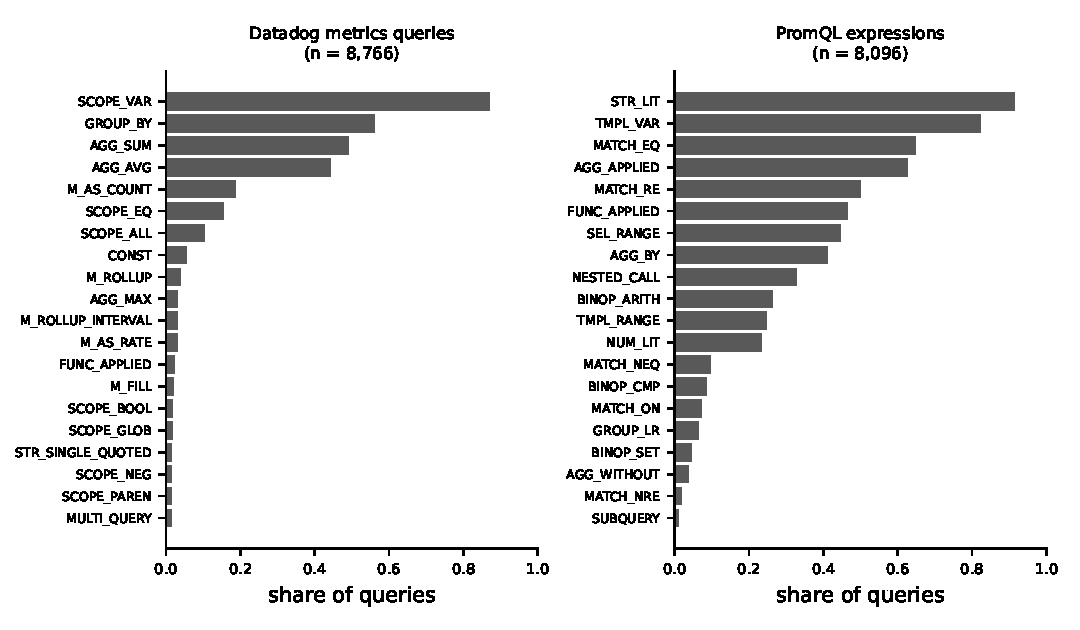
\includegraphics[width=\linewidth]{figures/feature_frequency}
\caption{The twenty most frequent structural features per language, as a share of
queries. Feature codes are those of \texttt{corpus.FEATURE\_DOC}; a query contributes to
every feature it uses.}
\label{fig:feature-frequency}
\end{figure}

\begin{table}[htbp]\centering\footnotesize
\begin{tabular}{@{}lllr@{}}
\toprule
Language & Kind & Name & Occurrences \\
\midrule
datadog & aggregator & \texttt{sum} & 4,480 \\
datadog & aggregator & \texttt{avg} & 4,057 \\
datadog & aggregator & \texttt{max} & 275 \\
datadog & aggregator & \texttt{count} & 58 \\
datadog & aggregator & \texttt{min} & 51 \\
datadog & aggregator & \texttt{p95} & 19 \\
datadog & function & \texttt{.as\_count} & 1,766 \\
datadog & function & \texttt{.rollup} & 331 \\
datadog & function & \texttt{.as\_rate} & 266 \\
datadog & function & \texttt{.fill} & 185 \\
datadog & function & \texttt{top} & 163 \\
datadog & function & \texttt{.weighted} & 70 \\
datadog & function & \texttt{per\_minute} & 27 \\
datadog & function & \texttt{per\_second} & 22 \\
datadog & function & \texttt{derivative} & 15 \\
datadog & function & \texttt{count} & 8 \\
promql & aggregator & \texttt{sum} & 4,718 \\
promql & aggregator & \texttt{max} & 718 \\
promql & aggregator & \texttt{avg} & 621 \\
promql & aggregator & \texttt{count} & 307 \\
promql & aggregator & \texttt{topk} & 230 \\
promql & aggregator & \texttt{min} & 84 \\
promql & function & \texttt{rate} & 2,541 \\
promql & function & \texttt{irate} & 1,078 \\
promql & function & \texttt{histogram\_quantile} & 507 \\
promql & function & \texttt{increase} & 328 \\
promql & function & \texttt{label\_replace} & 152 \\
promql & function & \texttt{vector} & 113 \\
promql & function & \texttt{sort\_desc} & 91 \\
promql & function & \texttt{label\_join} & 55 \\
promql & function & \texttt{time} & 50 \\
promql & function & \texttt{round} & 46 \\
\bottomrule
\end{tabular}

\caption{The six most frequent space aggregators and ten most frequent functions per
language, by occurrence. Datadog's \texttt{p}$NN$ percentile aggregators are five
distinct operators totalling $34$ occurrences, of which only \texttt{p95} reaches this
table.}
\label{tab:operator-frequency}
\end{table}

\noindent
Four things in these distributions are load-bearing for the rest of the paper.

\emph{Datadog's head is very short.} \texttt{sum:} and \texttt{avg:} are $95\%$ of all
every space-aggregator occurrence in Table~\ref{tab:operator-frequency}, and \texttt{by \{...\}} appears in $56\%$ of
queries. A translator that handles two aggregators and grouping already speaks most of
what the corpus says.

\emph{The counter rule that matters is the undivided one.} \texttt{.as\_count()} outnumbers
\texttt{.as\_rate()} by $6.6$ to one ($1{,}766$ against $266$). Both reduce to the same
cumulative difference by Proposition~\ref{prop:offset}, which is why that proposition,
rather than anything about \texttt{rate}, is the one that carries a migration.

\emph{PromQL's head is a rate.} \texttt{rate} and \texttt{irate} together are $69\%$ of
all $5{,}227$ function occurrences. Meanwhile subqueries appear in $1.1\%$ of PromQL
queries, \texttt{offset} in $0.3\%$, and the \texttt{@} modifier in none at all --- a
construct the language has and $8{,}096$ shipped expressions never reach for. The gap
between what a query language contains and what its users employ is itself part of the
switching-cost story: the hard parts of a language can be rare.

\emph{Nothing is used alone.} A real Datadog query combines a space aggregator, a scope
of several terms, a grouping and at least one method. That is why marginal frequency is
the wrong order to build a translator in, and why the next subsection reports a different
order.


\subsection{Coverage is a staircase, not a curve}
\label{sec:staircase}

A query is translatable only when \emph{every} feature it uses is supported, so for a
translator supporting exactly the feature set $S$, the share of queries all of whose
features lie in $S$ is an upper bound on $\kappa$. Choosing $S$ greedily --- at each step
the feature that completes the most queries outright --- gives an attainable set at each
size, hence a lower bound on the best ceiling a fragment of that size could reach.
Table~\ref{tab:implementation-order} is that order for Datadog and
Figure~\ref{fig:cumulative-coverage} both curves.

\begin{table}[htbp]\centering\scriptsize
\begin{tabular}{@{}rllrrr@{}}
\toprule
Step & Feature & Construct & Pending uses & Queries completed & Cumulative \\
\midrule
1 & \texttt{GROUP\_BY} & group by \{...\} & 4,922 & 20 & 1\% \\
2 & \texttt{MULTI\_QUERY} & comma-separated list of queries & 117 & 9 & 1\% \\
3 & \texttt{ARITH} & arithmetic between operands & 115 & 5 & 2\% \\
4 & \texttt{CONST} & numeric literal & 470 & 9 & 2\% \\
5 & \texttt{FUNC\_APPLIED} & function applied to the query & 205 & 1 & 2\% \\
6 & \texttt{AGG\_AVG} & space aggregator avg: & 3,885 & 1 & 2\% \\
7 & \texttt{SCOPE\_VAR} & dashboard template variable in the scope & 7,624 & 2,468 & 30\% \\
8 & \texttt{AGG\_SUM} & space aggregator sum: & 4,314 & 1,708 & 49\% \\
9 & \texttt{M\_AS\_COUNT} & .as\_count() & 1,644 & 1,079 & 62\% \\
10 & \texttt{SCOPE\_EQ} & scope term key:value & 1,347 & 974 & 73\% \\
11 & \texttt{SCOPE\_ALL} & scope \{*\} & 898 & 810 & 82\% \\
12 & \texttt{AGG\_MAX} & space aggregator max: & 275 & 245 & 85\% \\
13 & \texttt{M\_AS\_RATE} & .as\_rate() & 266 & 224 & 87\% \\
14 & \texttt{STR\_SINGLE\_QUOTED} & single-quoted string literal & 139 & 136 & 89\% \\
15 & \texttt{M\_FILL} & .fill(...) & 185 & 94 & 90\% \\
16 & \texttt{SCOPE\_GLOB} & wildcard in a scope value & 143 & 89 & 91\% \\
17 & \texttt{SCOPE\_NEG} & negated scope term !key:value & 134 & 91 & 92\% \\
18 & \texttt{M\_WEIGHTED} & .weighted() & 70 & 64 & 93\% \\
19 & \texttt{AGG\_COUNT} & space aggregator count: & 58 & 53 & 93\% \\
20 & \texttt{SCOPE\_BOOL} & boolean scope (AND / OR / NOT) & 160 & 37 & 94\% \\
\bottomrule
\end{tabular}

\caption{Greedy implementation order for Datadog. ``Pending uses'' is how many queries
still need the feature when it is chosen; ``queries completed'' how many it finishes on
its own. The cumulative column bounds $\kappa$ for a translator limited to those
features.}
\label{tab:implementation-order}
\end{table}

\begin{figure}[htbp]\centering
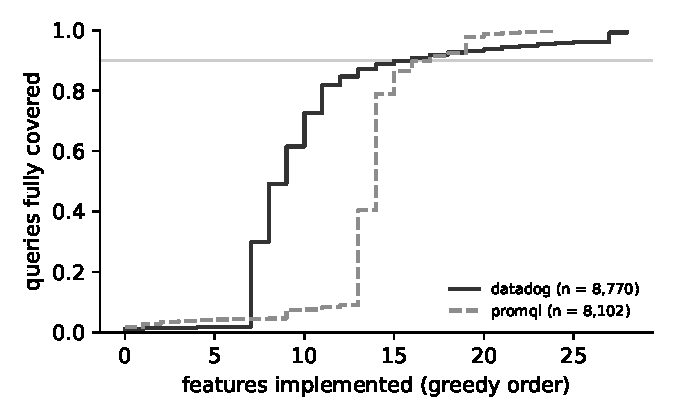
\includegraphics[width=0.62\linewidth]{figures/cumulative_coverage}
\caption{Queries fully covered against features implemented, in greedy order. The line
at $0.9$ marks the level reached after sixteen of Datadog's twenty-eight features and
seventeen of PromQL's twenty-four.}
\label{fig:cumulative-coverage}
\end{figure}

The shape is the finding. The first six Datadog features complete $45$ queries between
them --- $0.5\%$ of the corpus, on top of the $1.1\%$ that use no feature at all --- and
then template-variable scopes and \texttt{sum:} take two steps to $49.2\%$. Half the corpus
needs nine features; $90\%$ needs sixteen of the twenty-eight. PromQL behaves the same way
and slightly worse: its first six features complete $221$ of $8{,}102$ queries
($2.7\%$), half the corpus needs fourteen features and $90\%$ needs seventeen of
twenty-four.

For anyone building one of these translators this is the practical result of the paper. A
partial translator is worth almost nothing: there is no prefix of the feature list that
buys proportional coverage, because coverage is conjunctive over features while
popularity is marginal. The ``$80\%$ of queries with $20\%$ of the work'' intuition is
simply false here, and that asymmetry is a switching cost in its own right --- an
incremental migration cannot show incremental progress.


\subsection{What the unparsed queries are}

Six distinct queries ($8$ occurrences) are outside the grammar of
Section~\ref{sec:grammars}, and all six are the same construct: a conditional aggregator,
\texttt{count(v: v>=0):data\_streams.latency\{...\}}, which appears in Datadog's own
shipped dashboards and in none of its documentation. Writing a production for it would
mean guessing its semantics, so it is reported instead. It is the whole of the Datadog
residual in Table~\ref{tab:parse-coverage}.

\subsection{What is not measured}
\label{sec:not-measured}

Two of the facts this paper's rollup translations rest on are facts about Datadog's
implementation rather than about either language, and Datadog's documentation settles
neither. They are stated as assumptions in Section~\ref{sec:ingestion} and carried as
diagnostics in Table~\ref{tab:translation-caveats}. Both have since been settled, one of
them first from a source other than an experiment and then by one, and the difference
between the two kinds of evidence is worth keeping visible.

\emph{The reset policy $\rho$, settled by reading and then by measurement.} Datadog's
agent is open source, so what it does with a counter decrease is readable even though it
is undocumented: Remark~\ref{rem:rho} establishes $\rho=\mathsf{zero}$ for the
OpenMetrics ingestion path, which is what Proposition~\ref{prop:anchored} assumes. This
was not the expected answer. The prediction recorded in advance was
$\rho=\mathsf{drop}$, on which \emph{neither} candidate would have been exact across a
reset; the policy that the agent does implement alongside $\mathsf{zero}$ turns out to be
$\mathsf{clamp}$, and $\mathsf{drop}$ is not a reset policy at all.

Reading the agent does not establish that the backend stores what the agent sends, and
that step stood open longer than any other in this paper --- not for want of a design,
but because the experiment needs a counter that resets, and the replay of
Section~\ref{sec:replay} cannot supply one: a real request counter does not restart
inside half an hour. E1 supplies one on purpose. A scripted counter climbs to $1000$ and
drops to $100$ inside a single bucket while a real agent and a real Prometheus scrape the
same endpoint. Datadog stores $103$ over that bucket, which is $\delta_{\mathsf{zero}}$
and is distinct from what each of the three rivals predicts; and
\texttt{increase(x[$\Delta$] anchored)} over Prometheus returns $103$ for the same
bucket, on every complete bucket of all three counters. The restart rows of
Table~\ref{tab:rollup-live} therefore no longer stand on the model alone.

\emph{Bucket closure, settled by measurement.} $\Sigma_\Delta$ presumes a bucket
convention, and the one it presumed was wrong. Submitting a point on an exact bucket
boundary and another strictly inside one, then reading back which bucket each is reported
under, shows the buckets are left-closed and named by their \emph{start}
(Remark~\ref{rem:closure}); the two probes together leave one convention standing, and
each rival is ruled out by at least one of the two readings. It is one run at one rollup
interval, as \S\ref{sec:ingestion} says and this subsection used to deny by claiming two
runs at two intervals --- so what is pinned is the convention at $60$\,s rather than its
independence of the width. Epoch alignment itself \emph{is}
documented~\citep{ddrollup}; which edge the timestamp names was not.

No figure in this paper moved. A model and a candidate evaluated under the same
convention agree with each other, so what was wrong was a claim about Datadog rather than
any arithmetic --- Table~\ref{tab:rollup-live}, recomputed against a freshly re-verified
Prometheus on the corrected grid, is identical to the version computed under the wrong
one. What did change is where a translated query must be evaluated, and that is not a
detail: since a PromQL window is right-closed, no instant reads a left-closed bucket
exactly when a scrape lands on a boundary, and the translation must be evaluated strictly
inside the bucket. Evaluating on its right edge --- the obvious repair once the closure is
known --- is wrong on almost every bucket of an aligned scrape.

\emph{The corpus-scale differential test, no longer outstanding.} One further item
belonged in this subsection until recently, and it was the largest of them: the
construction of Section~\ref{sec:replay} applied to the whole corpus rather than to one
replayed trace. Until it ran, $\kappa$ measured what the translator was willing to
translate rather than what it translated correctly. It has since been run, and
\S\ref{sec:differential} reports it --- named rather than pointed at, because this
block is inline in one build and the last subsection of an appendix in the other,
where ``the next subsection'' was the references.



\texttt{UNSUPPORTED\_FUNCTION} is the largest and the least interesting: it is mostly a
bundle of Datadog functions the translator does not implement. \texttt{top(...)} leads
it at $139$ occurrences, and \texttt{per\_second(...)} follows at $22$.
Mostly, and not wholly: $11$ of its $208$ are not functions at all. Nine are a negated match-all,
\texttt{\{*,!*\}}, which is a scope and which the catalogue's own shortest example for
this row happens to be; one is a \texttt{.rollup(max)} over a known counter, which the
proof of Theorem~\ref{thm:kernel} classifies as a case where no rule exists rather than
as unwritten code; and one is a rollup whose \emph{width} is not numeric,
\texttt{.rollup(count, daily)}, refused where the interval is parsed rather than where a
function is looked up. All three stay in the unimplemented column, though the first of them for a duller
reason than \S\ref{sec:gaps} first gave: an earlier draft argued that PromQL can
denote an empty selection with a contradictory matcher pair and that \texttt{\{*,!*\}}
asks for one. The first is true and the second is false
(Remark~\ref{rem:empty-tag}) --- the term is discarded, and the exact translation is
to drop it. The individual deltas a
\texttt{max} rollup needs are reachable through a subquery over a sample grid the
query does not state --- the same omission the rollup interval makes everywhere else
--- and a
named calendar width is a unit the front end does not yet convert. Everything in it is now unimplemented
work and nothing else, which it was not when this section was first written: the
percentile aggregators sat in it as a genuine gap and \texttt{.weighted()} as a
supposed one, so the row was a mixture and the split at the end of this subsection had
to be computed by reading detail strings rather than codes. Both have moved ---
\texttt{.weighted()} out of the catalogue entirely (Remark~\ref{rem:weighted}) and the
percentiles into a code that names their obstruction.

The converse does not hold, and the comparison this subsection ends with depends on
noticing it: this row is not the whole of the unimplemented column. That column is now
five codes and $287$ occurrences --- this row's $208$, the four surviving disjunctions
below, the $36$ \texttt{FILL\_INTERPOLATION} occurrences Remark~\ref{rem:fill} moved
into it, and the $34$ \texttt{PHI\_QUANTILE} and $5$ \texttt{SCOPE\_EMPTY\_VALUE}
occurrences \S\ref{sec:gaps} moved into it last. This sentence read ``this row's $208$,
those four, and the $36$'' for as long as the column had held three codes, which sums to
$248$ and not to $287$: the last two retractions added their occurrences to the column
and not to the sentence describing it. One code has stopped being a mixture; the column
spans five, and it is the column rather than the code that the comparison is about.


\begin{remark}[\texttt{.weighted()} was the largest claimed gap and is not one]%
\label{rem:weighted}
Until recently this row was led by \texttt{.weighted()} at $70$ occurrences, described
here as ``a time-weighted space average that PromQL has no operator for''. That sentence
was the entire warrant, and it was wrong in both halves.

It is not an average: all $52$ distinct corpus forms attach the modifier to
\texttt{sum:}. An earlier version of this remark said $54$ of $56$ and conceded two
\texttt{avg:} uses; there are none. The count came from matching the substring
\texttt{weighted}, which also catches four queries whose \emph{metric name} contains it
and which carry no modifier at all --- two of them \texttt{avg:}, which is exactly the
concession. And it is not a gap, because it does not compute anything. A series
reporting at $0$, $50$ and $55$ seconds into each $60$\,s bucket has a plain mean of
$66.7$ and a mean weighted by the interval each point covers of $16.7$, so a rig built
on it can tell the two apart. Datadog returns $66.7$ with the modifier and without it,
on \texttt{GAUGE}, \texttt{COUNT} and \texttt{RATE} alike
(\texttt{scripts\slash weighted\_semantics.py}). The probe is narrower than that list
makes it sound, and the gap is worth naming: the grouped forms and the \texttt{sum} and
\texttt{avg} rollups were run on the gauge only, the counter types were probed
ungrouped under \texttt{avg}, and the modifier was never paired with a \texttt{count}
rollup at all. What closes that is not the probe but the corpus: three
\texttt{.weighted()} shapes went through the differential of \S\ref{sec:differential}
and agreed with Datadog bucket for bucket. On everything this corpus does with it,
\texttt{.weighted()} is the identity.

So the translation of a query carrying it is the translation of the query without it,
the front end drops the modifier as it already dropped \texttt{.fill(null)}, and $70$
occurrences move from the inexpressible column to $\kappa$. That is the third claimed
language gap in this paper to turn out not to be one, and the first to turn out not to
be work either: the other two were implemented, and this one needed deleting. The residue is a caution rather than a result: a modifier that does nothing
everywhere we can look may still do something somewhere we cannot, and what is measured
is every metric type and query shape the rig can build, not every configuration Datadog
has.
\end{remark}


\texttt{top(...)} decides where that split falls, so it is worth settling rather than
asserting. An earlier draft of this paragraph called it ``close to PromQL's
\texttt{topk}'', and that is false: Datadog ranks series by an aggregation over
\emph{all} values in the queried range and returns those series' whole trajectories,
while \texttt{topk} ranks independently at each evaluation instant, so a series can be in
one and not the other. They are different operators, and $139$ occurrences moving into
the inexpressible column would invert the comparison this section ends with.

They do not move, and the reason is instructive. PromQL \emph{can} denote the ranking,
using the \texttt{@} modifier to pin it to a single evaluation so that it does not drift
across the graph:
\begin{center}\footnotesize
\texttt{q and on($\overline{k}$) topk($n$, max\_over\_time(q[$R$] @ $T$))}
\end{center}
Read off a real Prometheus~3.15.0, this reproduces the selection that Datadog's
documented rule predicts --- aggregate each series over the whole range, take the top
$n$ --- and holds it constant across the range, while the naive \texttt{topk($n$, q)}
changes membership within the same workload at $n=2$
(\texttt{scripts\slash verify\_topk.py}; cached and regression-tested).
All $20$ cases agree: five ranking
functions, at $n=2$ and $n=3$, in both directions. The directions were the omission worth
finding. This corpus ranks ascending in $5$ of its $139$
occurrences, \texttt{topk} is the descending half of \texttt{top()}, and until
\texttt{bottomk} was asked for as well the measurement covered $134$ occurrences while
the sentence reporting it claimed $139$. The functions run the other way: the probe
covers five and the corpus uses four --- \texttt{mean} in $111$ of the calls,
\texttt{last} in $34$, \texttt{max} in $15$ and \texttt{sum} in $3$ --- so \texttt{min}
is probed because the candidate has to hold for it, not because a dashboard asks.

The Prometheus reading is one side of a comparison, and the other side of it was a
reading of Datadog's documentation --- the weaker kind of evidence, and the kind this
paper has twice found wrong, since the aggregation order and the bucket closure were both
read off the documentation and both wrong. So the vendor was asked the same question. The five series
go to a real Datadog as a gauge and \texttt{top()} itself is asked for its selection
(\texttt{scripts\slash datadog\_top.py}; cached and regression-tested), over the one
workload definition both scripts import so that the two halves cannot drift apart. All
$22$ selections are the ones the documented rule predicts, and two things the
documentation asserts rather than demonstrates are now readings as well. The selected
series come back over the \emph{whole} window and not only where they are winning: the
series that spikes once and then sits at $1$ returns all $20$ buckets, which is precisely
what a \texttt{topk}-shaped operator would not do. And the selection is relative to the
queried range --- over all twenty buckets the top two by \texttt{max} are the riser and
the spike, over the last ten the spike is outside the window and the answer is the riser
and the flat high series, while \texttt{mean}'s selection does not move under the same
narrowing. So \texttt{top(...)} is unimplemented work, and the catalogue's split stands.

What the expression costs is the interesting part, and that last reading is what prices
it. $R$ is the dashboard's time range and $T$ its end, and a Datadog query carries
neither --- the same omission as the rollup interval of \S\ref{sec:caveats}. That would
be a detail if the vendor's answer were insensitive to the range, and it is not: a
translator told the wrong range does not draw a slightly wrong graph, it selects
different series. An implementation of \texttt{top(...)} would therefore
reach the ceiling below only for a translator that is told the time range, and would
carry two more preconditions of exactly the kind \S\ref{sec:discussion} argues are the
real switching cost.

\texttt{PHI\_QUANTILE} ($34$) is the refusal this corpus comes closest to raising as an
information barrier in the main direction, and \S\ref{sec:ingestion} proves the
underlying fact rather than asserting it: a Datadog distribution metric answers
$\mathtt{p}NN$ from a sketch of the raw observations, Prometheus keeps those observations
bucketed with their sum and count, and no function of those is the quantile
(Corollary~\ref{cor:quantile}). The point is not that one system is more precise --- a
sketch is lossy too --- but that the two keep different lossy summaries of one stream and
neither recovers the other.

What this remark called ``one of the two information barriers this corpus raises'' it is
not, and the correction is \S\ref{sec:gaps}'s: the corollary's hypothesis is a
\emph{distribution} metric, and of the $34$ occurrences $20$ name metrics the vendor's
repository declares as something else, so the barrier does not apply to them. The
remaining $14$ name metrics the repository does not declare at all, which leaves them
undecided rather than blocked. So the sound reading of this refusal is a proved fact
about sketches and bucketings, a construct that fires on \texttt{p}$NN$ without testing
the fact's hypothesis, and $14$ occurrences where the hypothesis might hold and nothing
here says whether it does. PromQL's \texttt{histogram\_quantile} is not
the missing operator; it is a different approximation.


\begin{remark}[The second information barrier is in the label space]\label{rem:empty-tag}
\texttt{SCOPE\_EMPTY\_VALUE} ($5$) is the other, and it was found by reading
Lemma~\ref{lem:scope}'s proof rather than by any measurement this paper had taken. Datadog
separates three states of a tag: absent, present with an empty value, present with a
value. Prometheus's data model has two, because it \emph{defines} a label with an empty
value to be an absent label. Put to a real account on three series carrying
\texttt{k:v}, no \texttt{k} at all and \texttt{k:} respectively
(\texttt{scripts\slash scope\_empty\_tag.py}), all five scope forms behaved as that model
predicts:
\begin{center}\footnotesize
\begin{tabular}{@{}llll@{}}
\toprule
Scope & Datadog selects & Emitted matcher & which selects \\
\midrule
\texttt{!k:}  & \texttt{k:v}, no \texttt{k} & \texttt{k!=""}                      & \texttt{k:v} \\
\texttt{k:}   & \texttt{k:}                 & \texttt{k=""}                       & \texttt{k:}, no \texttt{k} \\
\texttt{k:*}  & \texttt{k:}, \texttt{k:v}   & \texttt{k=\textasciitilde{}".+"}    & \texttt{k:v} \\
\texttt{!k:*} & no \texttt{k}               & \texttt{k!\textasciitilde{}".+"}    & \texttt{k:}, no \texttt{k} \\
\bottomrule
\end{tabular}
\end{center}
Every row differs, and no PromQL selector closes any of them, because the distinction is
absent from what the target stores. The two bare forms are therefore refused: $5$
occurrences, all of \texttt{!k:}, which until this reading were translated as
\texttt{k!=""} and so dropped every series carrying no such tag --- the ordinary case, not
a corner one. The two glob forms are \emph{not} refused, because a rule does exist for
them: they are exact wherever no series carries that tag with an empty value, which is a
precondition the query cannot state and the translator therefore records, as
\texttt{TAG\_PRESENCE\_EMPTY} on $120$ occurrences ($1.4\%$ of the translated set) in
Table~\ref{tab:translation-caveats}. Refusing those $120$ would have been the
overcautious reading; an empty-valued tag is an odd thing for a real estate to carry, and
the honest report is the precondition rather than a $\bot$.

What this costs the paper is five occurrences off the ceiling --- a twentieth of a
point, at whatever the ceiling then stood at; the figures that bracketed it when this
remark was written were superseded by Remark~\ref{rem:fill} --- and what it appeared to
buy was the better half of the trade: a second construct that was inexpressible rather
than unbuilt, measured against the vendor, in a direction \S\ref{sec:ingestion} argues is
nearly free of information loss.

That half of the trade did not survive, and the reason is in this remark already. If
dropping the term is the exact translation of \texttt{k:*} on $120$ occurrences, it is
the exact translation of \texttt{!k:} on these five, and \S\ref{sec:gaps} now counts
them as work rather than as a barrier --- so ``nearly'' is carrying one exception again,
and the direction is as free of information loss as the remark said before it argued
itself out of the claim. What the measurement still buys is the $120$, and a sharper
lesson than the one intended: the overcautious reading was available on both sides of
the same line, and this remark took it on one of them.
\end{remark}


\texttt{LABEL\_NAME\_GLOB} ($31$) is the one clean expressiveness case left, and with
\texttt{.weighted()} withdrawn, the disjunctions reclassified and
\texttt{FILL\_INTERPOLATION} returned by Remark~\ref{rem:fill}, it and the percentiles
and the empty-valued scopes are all that remains. A wildcard in a tag \emph{key} rather
than a value, as in \texttt{\{*-location\}}, asks for a match over label \emph{names},
which a PromQL selector cannot do, because label names are not queryable there ---
Remark~\ref{rem:label-name} puts that to a real server, including the quoted-name
syntax 3.x added, which looks like somewhere a pattern could go and is not.

This paragraph used to argue the fill row as well, and the argument it used is the one
Remark~\ref{rem:fill} broke: that a PromQL expression has no term introducing a sample
where the database holds none, with \texttt{or vector(0)} offered as the nearest thing
and correctly rejected for supplying one unlabelled series rather than a value per
series. The rejection was right and the generalisation was not. What survives of the
paragraph is the observation it made in passing, which turns out to have been the more
useful one: the code's name never fitted its contents. Datadog's interpolating modes
are \texttt{.fill(linear)} and \texttt{.fill(last)}, and this corpus holds one
\texttt{last} and no \texttt{linear} at all --- the other $35$ are constant fills. The
row was named for a construct the corpus does not contain, and a name is a poor thing
to argue from.

\texttt{SCOPE\_DISJUNCTION} is the interesting row, and it is interesting for having
almost emptied. A Datadog scope is a boolean query over tags
(Figure~\ref{fig:productions}) and a PromQL selector is a \emph{conjunction} of matchers,
so disjunction is the one scope operator with no selector-level form --- unless every
branch constrains the same tag key, in which case Proposition~\ref{prop:disjunction}
makes it a single regex matcher. An earlier version of this translator refused all of
it, at $124$ occurrences, and reported that as a gap in the language. It was not: $120$
of those occurrences are single-key disjunctions, and implementing
Proposition~\ref{prop:disjunction} translates them, taking $\kappa$ from $94.2\%$ to
$95.6\%$ at the time, and $96.6\%$ as it now stands.

What survives is four occurrences: disjunction across
different keys (\texttt{\{(status:400 OR s)\}}), a branch that constrains two keys at
once (\texttt{\{(a:1 AND b:1) OR (a:2 AND b:2)\}}), and one De~Morgan case that becomes
the same thing. Those remain sayable in PromQL as a union of selectors, but not as the
syntax-directed translation of a scope --- which is why the split below counts them as
unfinished work rather than as a language gap. That expressibility claim is held to a
weaker standard than the one \texttt{top(...)} is held to, and
the asymmetry should be visible rather than quietly enjoyed: the union there was
written out and read off a real server, while this one is sketched and never built, so
what moves these four occurrences into the engineering column is an argument rather
than a reading. Four occurrences do not move the split, but the standard is the point
of the split. An earlier version of this section put
them in the inexpressible column, where they contradicted the sentence above that says
PromQL expresses them; a property of this translator's architecture is not a property
of the target language.

The episode is worth recording rather than quietly fixing, because the mistake is the
one this paper is most at risk of making throughout. A translator's refusal looks like
evidence about the languages, and it is only evidence about the translator until
something separates the two. Here what separated them was re-parsing the refused queries
and asking which case each was --- a question the gap code alone could not answer, since
one code covered both.

\begin{table}[htbp]\centering\footnotesize
\begin{tabular}{@{}llrr@{}}
\toprule
Feature & Construct & Occurrences & Translated \\
\midrule
\texttt{AGG\_COUNT} & space aggregator count: & 58 & 0.0\% \\
\texttt{FUNC\_APPLIED} & function applied to the query & 205 & 0.0\% \\
\texttt{SCOPE\_BARE} & scope term that is a bare tag key & 92 & 0.0\% \\
\texttt{STR\_SINGLE\_QUOTED} & single-quoted string literal & 139 & 0.0\% \\
\texttt{SCOPE\_PAREN} & parenthesised scope & 122 & 0.0\% \\
\texttt{SCOPE\_IN} & scope membership test IN (...) & 51 & 0.0\% \\
\texttt{M\_WEIGHTED} & .weighted() & 70 & 0.0\% \\
\texttt{AGG\_MAX} & space aggregator max: & 275 & 4.0\% \\
\texttt{SCOPE\_BOOL} & boolean scope (AND / OR / NOT) & 160 & 14.4\% \\
\texttt{AGG\_MIN} & space aggregator min: & 51 & 35.3\% \\
\texttt{CONST} & numeric literal & 470 & 62.8\% \\
\texttt{M\_FILL} & .fill(...) & 185 & 63.2\% \\
\bottomrule
\end{tabular}

\caption{The twelve features with the lowest translated share, among those appearing in
at least $50$ query occurrences. Rows read ``queries using this feature'', not ``this
feature''.}
\label{tab:gap-by-feature}
\end{table}

Table~\ref{tab:gap-by-feature} attributes the refusals to the Datadog features the
refused queries use, and the caveat in its caption is load-bearing. A feature at $0.0\%$
is not necessarily one the translator cannot handle; it can be one that in this corpus
only ever appears beside something else that fails. \texttt{SCOPE\_BARE} demonstrated
this and then stopped: \texttt{avg:x\{host\}} alone translates to
\texttt{x\{host=\textasciitilde{}".+"\}}, yet before
Proposition~\ref{prop:disjunction} the feature stood at $0.0\%$, because in these
dashboards a bare tag key occurs only inside a boolean scope or next to a
\texttt{*-location} key glob. Translating the scopes moved it to $83.6\%$ without anyone
touching bare tag keys. Reading such a row as a statement about its own feature would
have overstated the gaps, which is why the gap catalogue and not this table is the
claim.


\paragraph{How much of the shortfall is beyond reach.}
Separating the kinds of refusal is the point of having codes at all, and on this corpus
the separation has an answer this paper did not set out to report: none of it is beyond
reach. Three kinds are possible and the catalogue keeps them apart --- what Prometheus
does not \emph{hold}, what PromQL cannot \emph{say}, and what this translator has not
\emph{built} --- with a fourth, a query Datadog itself rejects, which
Remark~\ref{rem:third-refusal} describes and which is empty here too. The first two
columns are empty. All $287$ refused occurrences, $3.3\%$ of the corpus, are constructs
this translator has not implemented, \texttt{top(...)} chief among them.

The column did not start empty, and \S\ref{sec:discussion} keeps the running count of
what left it and why, because the pattern is more informative than the total. The last
three to go were the percentile aggregators ($34$), the tag-key globs ($31$) and the
scopes separating an absent tag from one present with an empty value ($5$): a corollary
applied where its own hypothesis fails, a construct this paper's normaliser fabricated
out of a template variable, and an information barrier that turns out to decide the
translation rather than to block it.

Because a query is abandoned at its first obstruction (Remark~\ref{rem:one-gap}),
$99.9\%$ is an upper bound on what implementing the unimplemented set would reach rather
than a promise: a refused query could carry a second obstruction behind the first.
Re-reading the $287$ for the other codes' constructs finds none, so the bound is tight
with nothing left over. What separates it from $100\%$ is not a construct at all --- it
is the $8$ occurrences \S\ref{sec:grammars}'s grammar does not parse, which is a fact
about this paper's instrument and not about either language. Against the $96.6\%$
measured here, the whole distance to the ceiling is engineering, as the disjunction rule
demonstrated by closing $1.4$ points of it and \texttt{.weighted()} by closing $0.8$
more. That is the finding to carry into \S\ref{sec:discussion}: going this way, the
apparent incompatibility is work, all of it, and what is left over is small enough to
enumerate query by query.


\begin{remark}[What the assumed interval costs, measured]\label{rem:rollup-default-cost}
How much that costs is now measured rather than left open. Asked of a real account, the
interval a bare query receives is a function of the query range: $20$\,s over an hour,
$60$\,s over four hours, $300$\,s over a day, monotone in between
(\texttt{scripts\slash trial\_checks.py e4}). The translator assumes $60$\,s, so it is
exactly right for a four-hour dashboard and wrong by a factor of three for the one-hour
view --- and the window width is not a detail, since it is the $\Delta$ in every rollup
rule of \S\ref{sec:ingestion}. The assumption is therefore not unverified but
\emph{conditional}, and the condition is a dashboard setting no query carries. Asking for
a finer interval than the range allows is refused outright rather than silently widened,
which is the better of the two behaviours for a translator: the limit is on points
returned per query, so the error is visible instead of the data being quietly coarser
than asked for.
\end{remark}

\begin{remark}[Two conditions that coincide in this corpus without being one]\label{rem:counter-caveats}
\texttt{COUNTER\_RESET} marks the $23.6\%$ that use the cumulative-difference form of
Proposition~\ref{prop:offset}, exact unless a counter resets inside the window;
Table~\ref{tab:rollup-live} measures what that costs when one does, and
Proposition~\ref{prop:anchored} removes it at the price of a server started with an
experimental feature enabled --- a stronger condition than a version number, and
Remark~\ref{rem:anchored-flag} is about how we came to believe otherwise.

\texttt{PHI\_SERIES\_START} marks the same $23.6\%$, and marks it for a second reason
that went unrecorded until this draft. The cumulative difference needs a sample
\emph{before} the bucket to subtract, and a series younger than the window has none, so
the expression returns no result where Datadog returns the deltas it does hold
(Remark~\ref{rem:series-start}). The code existed from the start --- it was written for
the reverse direction --- and the counter rules had been emitting without it. The two
shares coincide because in this corpus the same translations carry both: every counter
rule here is the cumulative difference, which needs a predecessor sample and a
reset-free window alike. They are not the same condition, and the anchored form
separates them --- it discharges both for a $\mathsf{sum}$ rollup, and only the reset
one for the mean-of-deltas rule, whose denominator counts samples where Datadog counts
deltas however the numerator is written. Where it does discharge both, its
experimental-flag requirement is a better bargain than
Remark~\ref{rem:anchored-flag} alone suggests.
\end{remark}

\begin{remark}[The caveat that was missing, and what it is worth]\label{rem:type-caveat}
\texttt{METRIC\_TYPE\_UNKNOWN} is new to this table and is the reason to report caveats at
all rather than to list them once in prose. An \texttt{avg}, \texttt{min}, \texttt{max} or
\texttt{count} rollup reduces the points Datadog stores, which are samples for a gauge and
per-interval deltas for a counter; the emitted \texttt{*\_over\_time} is exact for the
first and unrelated to the second, and a dashboard does not record which it is
(Remark~\ref{rem:gauge}). At $100\%$ of translated occurrences it is the largest
qualification here, and it was missing from this table until the soundness theorem of
Section~\ref{sec:kernel-soundness} was written down and its hypotheses compared against
what the emitter actually recorded. It reached $100\%$ later still: the quarter of
translations that use \texttt{.as\_count()} or \texttt{.as\_rate()} were held to
establish their own metric type until the modifiers were measured on a gauge and found to
be silent no-ops (Remark~\ref{rem:gauge}). $\kappa$ did not move when it was added --- the
expressions are the same ones --- which is exactly why it is worth having: an unrecorded
precondition costs nothing in any number the paper reports, right up to the point where
somebody relies on the translation.

How often it is \emph{violated} is now measured rather than left as a worry, and it is
the one place in this paper where a precondition turns out to fail at a rate worth
reporting. The repository the dashboards come from declares each metric's type in a
file the corpus fetch had passed over, which settles the question for $7{,}557$ of the
$8{,}444$ translated occurrences --- $89.5\%$. On $491$ of those the front end's
inference disagrees with the declaration: $6.5\%$ of the decidable set and $5.6\%$ of
the corpus, split $242$ counters translated as gauges and $249$ gauges translated as
counters (Remark~\ref{rem:type-measured}). So $\kappa$ counts those $491$ among its
translations and they are, on the vendor's own declaration, wrong. $\kappa$ is a
coverage measure and was never a correctness measure; this is the first number in the
paper that says how far apart the two are.

Adding it also falsifies something an earlier draft of this section claimed. That draft
said $116$ occurrences carried \texttt{ROLLUP\_ALIGNMENT} alone and were the only
translations resting on nothing but the grid. With this code in place the true
figure is \emph{none}: every one of those $116$ is an \texttt{avg} rollup and now carries
\texttt{METRIC\_TYPE\_UNKNOWN} too. No translation in this corpus is exact on the strength
of the evaluation grid alone, which is a stronger claim than the one it replaces and was
only invisible because a precondition was. The same correction then ran to its conclusion:
with the modifiers' evidential value withdrawn, no translation in this corpus is exact on
the strength of anything the query itself contains.
\end{remark}

\begin{table}[htbp]\centering\scriptsize
\begin{tabular}{@{}lll@{}}
\toprule
Feature & Datadog & PromQL \\
\midrule
\texttt{M\_AS\_COUNT} & \texttt{sum:esxi.vm.count\{*\}.as\_count()} & \texttt{sum(esxi\_vm\_count - esxi\_vm\_count offset 60s)} \\
\texttt{M\_AS\_RATE} & \texttt{sum:n8n.cache.hits.count\{*\}.as\_rate()} & \texttt{sum((n8n\_cache\_hits\_count - n8n\_cache\_hits\_co\dots{}} \\
\texttt{M\_ROLLUP\_INTERVAL} & \texttt{avg:mongodb.uptime\{*,*\}.rollup(avg, 60)} & \texttt{avg(avg\_over\_time(mongodb\_uptime[60s]))} \\
\texttt{GROUP\_BY} & \texttt{fluentd.retry\_count\{*\} by \{host\}} & \texttt{avg by (host) (avg\_over\_time(fluentd\_retry\_co\dots{}} \\
\texttt{SCOPE\_NEG} & \texttt{sum:iis.errors.locked\{!site:total,*\}} & \texttt{sum(avg\_over\_time(iis\_errors\_locked\{site!="to\dots{}} \\
\texttt{SCOPE\_GLOB} & \texttt{sum:snmp.devices\_monitored\{agent\_host:*\}} & \texttt{sum(avg\_over\_time(snmp\_devices\_monitored\{agen\dots{}} \\
\texttt{ARITH} & \texttt{-sum:tomcat.bytes\_rcvd\{*\}} & \texttt{-sum(avg\_over\_time(tomcat\_bytes\_rcvd[60s]))} \\
\bottomrule
\end{tabular}

\caption{Worked translations, each the shortest corpus query exercising that feature.
Long expressions are truncated.}
\label{tab:translation-examples}
\end{table}

\noindent
Table~\ref{tab:translation-examples} shows what the output looks like, taken from the
corpus rather than invented. The \texttt{M\_AS\_COUNT} row is Proposition~\ref{prop:offset}
in use; the \texttt{GROUP\_BY} row shows the default time aggregator and the assumed
interval together, which is the common case.

\begin{remark}[Why the differential is a smaller experiment than it looks]\label{rem:shape-reduction}
It is a smaller experiment than it looks, which is worth recording because the obvious
estimate is badly wrong. It does not need every metric the corpus names to exist in both
systems. What a differential test exercises is the \emph{operator structure} --- which
rollup, which aggregation, which matcher shapes --- and two queries that differ only in
the metric they name are one experiment, not two. The abstraction takes out the
identifiers and nothing else --- metric names, tag keys, tag values, and the content of
regex matchers, whose own conversion \S\ref{sec:regular} decides separately --- and what
a query would \emph{emit} differently is kept: the rollup interval, a scale factor and a
numeric literal all survive it. That matters, and it did not hold until the seventh
reading of this apparatus. The interval used to collapse to whether one was stated at
all, which put $70$ occurrences into this experiment under a window width they do not
state and two of them under a width the rig cannot hold two buckets of; the congruence
check below could not see it, because it masked digits along with identifiers and
\texttt{[15s]} and \texttt{[300s]} mask alike. Abstracting that much collapses the
$8{,}370$ translated occurrences that are
a single query to \textbf{$332$ distinct shapes}, and they are as unevenly distributed as
everything else in this corpus: $6$ shapes cover half the occurrences, $23$ cover $80\%$,
$50$ cover $90\%$ and $107$ cover $95\%$. A median query has one metric slot and two tag
keys, so at three label values apiece the whole set came to $885$ synthetic
series --- a scale a single trial account sustains, which is why the experiment turned
out not to need a reconstruction of somebody's production estate. The reduction is only
sound if every query in a class translates the same way, and that is checkable rather
than arguable: emitting all of them and masking the identifiers leaves each class with
exactly one form, so a representative stands for its class. Establishing
that found a wart worth fixing --- the emitter decided parenthesisation by scanning its
own output for operators, so a hyphen inside a tag value such as \texttt{result:hit-wait}
was read as one and wrapped the expression in parentheses that meant nothing.
\end{remark}

\begin{remark}[Three preconditions of the run that were wrong]\label{rem:differential-fixes}
Three preconditions of this run were wrong in the version of it reported before the
seventh reading of the apparatus, and all three made agreement easier to obtain. The
scrape grid began at an arbitrary whole second, and off a bucket boundary a left-closed
Datadog bucket and a right-closed PromQL window hold the same samples --- so the
evaluation instant could have been wrong by up to half a scrape and still agreed on every
bucket, which makes the one convention this paper got wrong in draft the one the
corpus-scale test was silent about. It is now floored to a multiple of $300$\,s, which is
a multiple of every interval this corpus states below the run's window, so the samples
land on boundaries and the instant is load-bearing. A scope requiring a tag merely to be
\emph{present} pinned that tag to one value, so eight shapes grouping by the very key
they test for presence were compared over a single series and their space aggregation was
never exercised. And the rollup interval was not part of a shape, so $70$ occurrences were
tested at a window width they do not state. All three are fixed, the shape count rose
from $325$ to $335$ as the finer abstraction split six classes, and then to $332$ when
the empty-value scopes of Remark~\ref{rem:empty-tag} left the translated set, and the
agreement did not
move: $329$ of $329$, on a grid where the closure convention is visible and where every
occurrence is tested at its own width. Those are that run's figures; the third run, on a
third independent set of series and with the grouping-key fix in place, reports $330$ of
$330$ over $333$ shapes. One of those is the \texttt{velero} query whose scope
\texttt{corpus.\_TMPL} used to truncate at its first hyphen (\S\ref{sec:gaps}):
instantiated correctly it groups by the four keys it names and compares bit-identically,
so the normaliser defect that had filed $31$ occurrences as beyond reach had also been
keeping a shape out of this experiment. A defect in one instrument is rarely confined
to the figure it was found in. The one occurrence class the fix removed rather
than repaired is the second \texttt{window-too-short} row --- a $3600$\,s rollup, which
the old abstraction had folded in with $300$\,s and credited as agreeing, and which this
rig provably cannot hold two buckets of.
\end{remark}

\begin{remark}[Six systematic failures, every one the harness]\label{rem:harness-failures}
Six systematic failures came out of this rig and every one was the harness rather than
the systems: three had to be cleared before any of the four defects was visible at all,
and three more surfaced as the run was tightened. That ratio is the honest summary of
the exercise, and a more useful lesson about differential rigs than the agreement rate
is. Metric names shared across runs let Datadog see two runs' points where Prometheus
saw one, which looked like a uniform $30\%$ error. A global $60$~s bucket grid compared
a \texttt{.rollup(sum, 300)} bucket against a PromQL window covering a fifth of its
span, which looked like $21$ broken shapes. Reading a group's value off the query's
scope rather than the response's tag set took the glob the query asked for instead of
the value it matched, which looked like $32$ shapes whose groups did not line up. Tag
keys containing dots were submitted in PromQL's normalised spelling while the Datadog
query still asked for the dotted one, so Datadog grouped by a tag that was not there ---
and the fix for it was a regex over the query text, which was blind to hyphens, so the
same fault survived in the one shape of \S\ref{sec:differential} that the second run
reported \texttt{unmatched}; it is off the parse tree now. A
scope term requiring a tag to be non-empty was satisfied by leaving the tag off, which
Prometheus reads as empty, so that side selected nothing. And a rate limit from the API
was recorded as a shape that could not be compared. In every case a parameter was read
from somewhere other than the place that stated it --- which is the same sentence as
\S\ref{sec:caveats}'s, about a rig instead of a query.
\end{remark}

\begin{remark}[What the run does not cover]\label{rem:differential-limits}
The run does not cover everything, and Table~\ref{tab:differential} says so rather than
quietly dropping what it misses. One shape states a $1800$~s rollup, which the run's
half-hour window cannot hold two of. One asks for a tag to equal \texttt{5} and match
\texttt{4*} at once, which no series satisfies, so both systems correctly return nothing
and there is nothing to compare. The data is synthetic: the shapes are the corpus's, the
series are not, so the test exercises operator structure and not the distributional
oddities of real traffic --- which is what Section~\ref{sec:replay}'s replay of a real
trace is for, and the two are complementary rather than redundant.
\end{remark}

\begin{remark}[Three ways to write a string, and the counts that missed two]\label{rem:string-forms}
The three-way split of Table~\ref{tab:regex-glob} rose in the seventh reading of the
apparatus, and the table's own caption is why: it says ``every
\texttt{=\textasciitilde{}} and \texttt{!\textasciitilde{}} matcher'', and the scanner
behind it accepted only double-quoted patterns. PromQL writes a string three ways, its
own grammar in Section~\ref{sec:grammars} says so, and $114$ matcher occurrences sat in
the other two. The caption was the instrument that found it: a claim stated over
\emph{every} matcher is falsifiable by a matcher, where one stated over the matchers the
scanner happened to read is not.
\end{remark}

\noindent
Before the split is trusted it is worth seeing what each of its three classes
contains. Table~\ref{tab:regex-glob-examples} is that, and the patterns are the kind
each class name suggests --- the cheapest available check that the classifier is
classifying what it claims to.

\begin{table}[htbp]\centering\footnotesize
\begin{tabular}{@{}llr@{}}
\toprule
PromQL regex & Datadog scope value & Occurrences \\
\midrule
\texttt{\textasciicircum{}k8s\_.*} & \texttt{k8s\_*} & 60 \\
\texttt{.*external-dns.*} & \texttt{*external-dns*} & 36 \\
\texttt{.*pod.*} & \texttt{*pod*} & 24 \\
\texttt{LIST|GET} & \texttt{GET, LIST} & 41 \\
\texttt{ext.*|xfs} & \texttt{ext*, xfs} & 34 \\
\texttt{proxy|attach|log|exec|portforward} & \texttt{attach, exec, log, portforward, p\dots{}} & 32 \\
\texttt{.+} & $\bot$ No non-empty wildcard & 133 \\
\texttt{(/dev/)?(mmcblk.p.+|nvme.+|rbd.+|\dots{}} & $\bot$ No non-empty wildcard & 49 \\
\texttt{5..} & $\bot$ No single-character wildcard & 40 \\
\bottomrule
\end{tabular}

\caption{The three most frequent regular expressions of each outcome.}
\label{tab:regex-glob-examples}
\end{table}

\begin{remark}[What the cross-check cost, and which patterns cost it]\label{rem:crosscheck-timing}
An earlier version of this paragraph reported $168$ of $183$ and recorded the remainder
as not reached, which was a statement about a clock rather than about the procedure. The
script takes a time budget, that run was given $2{,}400$\,s, and four patterns of one
family --- a parenthesised alternation inside a long literal, as in
\texttt{cnpg\_pg\_stat\_(bgwriter|checkpointer)\_checkpoints\_timed} --- cost $91$ to
$176$ seconds each when timed on an idle machine, so the budget expired partway through
them. Run without one the cross-check takes $2{,}998$\,s and finishes. What makes those
patterns expensive is worth naming, because it is the procedure working rather than
struggling: the shortest word of such a pattern is forty-odd characters, so the pruned
space of star insertions is large, and the search has to \emph{exhaust} it to conclude
that no single glob exists. The costly cases are the negative ones, and they are exactly
the cases a structural proposer's refusal would otherwise have to be taken on trust. The run is cached
(\texttt{scripts\slash crosscheck\_globs.py}), and \texttt{tests\slash test\_regular.py}
fails if a disagreement ever appears, if any pattern goes unreached, or if the two sides
stop sharing a population.
\end{remark}

